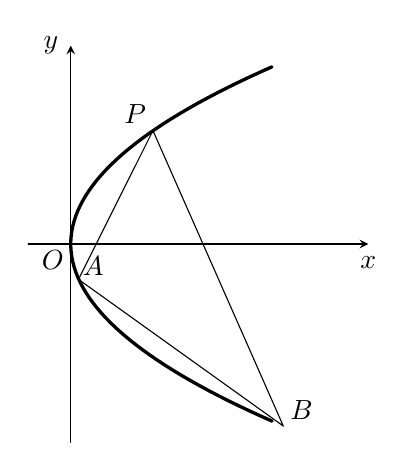
\begin{tikzpicture}[>=stealth, scale=0.9, line cap=round, line join=round]
  % Axes
  \draw[->] (-0.6, 0) -- (4.2, 0) node[below=1pt] {$x$};
  \draw[->] (0, -2.8) -- (0, 2.8) node[left=1pt] {$y$};
  \node[below left=-1pt] at (0, 0) {$O$};

  % Parabola x = y^2 / 2.2
  \draw[very thick] plot[domain=-2.5:2.5, samples=70] ({(\x)^2 / 2.2}, \x);

  % Coordinates
  \coordinate (P) at (1.16, 1.6);
  \coordinate (A) at (0.11, -0.5);
  \coordinate (B) at (3.0, -2.57);

  % Triangle PAB
  \draw (P) -- (A) -- (B) -- cycle;

  % Labels
  \node[above left=-1pt] at (P) {$P$};
  \node[above right=-2pt] at (A) {$A$};
  \node[above right=-1pt] at (B) {$B$};
\end{tikzpicture}
